%&latex
\documentclass[msc, openright, a4paper]{TNthesis}

%package declaration 
\usepackage{times}
\usepackage{paralist}
\usepackage{graphicx}
\usepackage{indent}  
\usepackage{listings} 
\usepackage{rotating}
\usepackage{color} 

\title{Enabling Distributed Programming Abstractions for Real-World
Wireless Sensor Networks (draft)}

\author{Galiia Khasanova}

\newcommand\B{\rule[-1.7ex]{0pt}{0pt}} % Adds a space between the text and the [B]ottom \hline
\newcommand\T{\rule{0pt}{3.1ex}} % Adds a space between the text and the [T]op \hline


\abstract{
 This thesis presents blah blah blah.
 }
\begin{document} 

\begin{preliminary}
\maketitle 

\standarddeclaration

\begin{acknowledgements}
	Bla
\end{acknowledgements}

\begin{acronyms}
	\begin{center}
	\begin{tabular}{| l |p{9cm}|}
	\hline
	ADT \T \B & Abstract Data Type \\
	\hline
	CLDC \T \B & Connected Limited Device Configuration \\
	\hline
	DADT \T \B & Distributed Abstract Data Type \\
	\hline
	Java ME \T \B & Java Micro Edition \\
	\hline
	JiST \T \B & Java in Simulation Time \\
	\hline
	JVM \T \B & Java Virtual Machine \\
	\hline 
	LN \T \B & Logical Neighborhoods \\
	\hline
	MAC \T \B & Media Access Control \\
	\hline
	OS \T \B & Operating System \\
	\hline
	RF \T \B & Radio Frequency \\
	\hline
	Sun SPOT \T \B & Sun Small Programable Object Technology \\
	\hline
	SWANS \T \B & Scalable Wireless Ad hoc Network Simulator \\
	\hline
	VM \T \B & Virtual Machine \\
	\hline
	WSN \T \B & Wireless Sensor Network \\
	\hline
	WSAN \T \B & Wireless Sensor and Actor Networks \\
	\hline
	\end{tabular}
	\end{center}
\end{acronyms}


%\dedication{To Eric Cartman, Southpark, Colorado, USA. Only because my
%boyfriend insists.}
\tableofcontents
\listoffigures
\listoftables
\end{preliminary} 


\chapter{Introduction}

\textcolor{green}{Jo: quote is fine, but better Sth Like : Mark Weiser once
wrote in his visionary paper from whenever [22]:}

\begin{quote}
\emph{``The most profound technologies are those that disappear. They weave
themselves into the fabric of everyday life until they are indistinguishable
from it''} 
Mark Weiser \cite{Weiser_ComputerIn21stCentury}
\end{quote}


\textcolor{blue}{some intro words here.. .. and later stuff about .. The chapter
begins with an introduction to wireless sensor nodes and Wireless Sensor Networks (WSNs). This is followed by a
description of the protocol stack used in this work}



\section{Introduction to Wireless Sensor Networks}

Recent advances in micro system technologies and wireless communication
made it possible to deploy wireless sensor networks (WSNs) that contain a large
number of sensor nodes, multifunctional devices characterised by their low- cost,
low-power, and small form factor, that can communicate across short distances
using Radio Frequency (RF) communication \cite{SensorSurveyAkyildiz:2002}.

WSNs are being used in a wide range of applications in military and civilian
operations such as, for instance, health monitoring, environment monitoring,
data acquisition in dangerous environments, and target tracking.

This chapter begins with the introduction of sensor nodes and
discussion over followed by presentation of the most important features of WSNs.

\subsection{Sensor Nodes} \label{subsec:sensornodes}

Typically, a sensor node consists of the following elemants (as it can be seen
from the Figure \ref{Fig:SensorNodeArch})
\begin{itemize}
  \item \emph{Sensing unit}, which is comprised of a number of sensors and
  analog-to-digital converters. 
  \item \emph{Tranceiver}, which facilitates node-node communication using 
a variety of techniques.
  \item \emph{Processing unit}, that usually comprises a 
microcontroller/microprocessor that performs processing, and is associated with 
a storage unit.
  \item \emph{Power unit}, which provides the energy required to run the sensor node, and can use chemical 
batteries or power scavenging units such as solar cells.
\end{itemize}


\begin{figure}
\centering
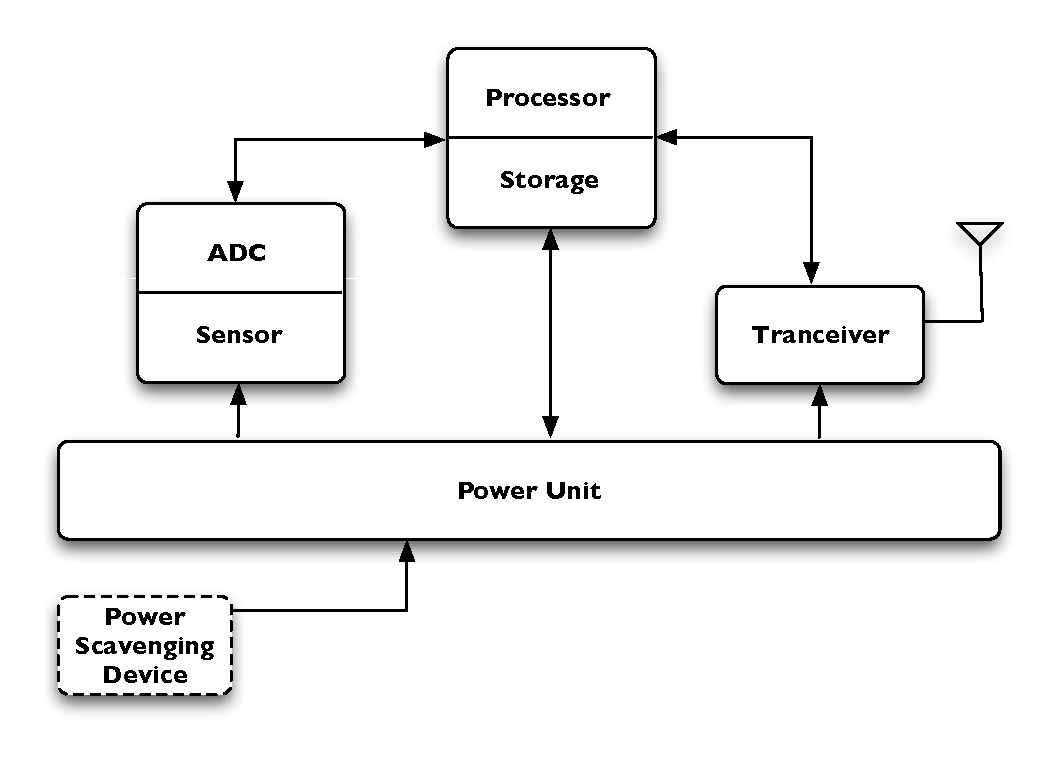
\includegraphics[scale=0.65]{img/SensorNodeArch.eps} 
\caption[Architecture of a sensor node] {Architecture of a sensor node (adapted from \cite{SensorSurveyAkyildiz:2002}).}
\label{Fig:SensorNodeArch}
\end{figure} 


\textcolor{green}{the next paragraph needs a bit of reformulation. about the constraints
I think your argumentation should go like size/weight -> battery  (that's the
point where it really gets hard to make smaller). -> energy efficient processing, memory and so on
and cost as an additional constraint }

Sensor nodes have constraints on both their size and their cost. The former 
constraint arises from the requirement that sensor nodes be easily deployable, 
while the latter arises from the requirement for fault tolerance (which in turn 
can be achieved only by being able to deploy cost-effectively large numbers of
sensor nodes in the environment being monitored). These limit the memory capacity, processing 
power, and the amount of energy available on a particular node.

\subsection{Wireless Sensor Networks}
\textcolor{green}{the first sentence of 2.1.2 is a bit well, almost German
too long and self referring. actually, what you write about in that section, is more like routing in networks of sensor nodes
maybe you should expand a bit}

As mentioned in the previous section, sensor nodes are capable of communicating
untethered with one another, and hence are capable of forming networks of nodes
called a Wireless Sensor Network. 

WSNs are typically deployed randomly in an
environment where phenomena are required to be monitored. 

A WSN is self-organising system, given the random nature of the deployment.

Its topology is subject to change, and therefore sensor nodes should be
capable of dealing with changes of this kind in order to cope with hostile
operating conditions, the failure-prone nature of sensor nodes and the possibility of 
redeployment of additional sensor nodes at any time during operation.


\section{WSN Protocol Stack} \label{sec:WSNProtStack}

The WSN protocol stack presented in \cite{SensorSurveyAkyildiz:2002} is adapted
from \cite{ComputerNetworksTannenbaum:2003}. As it can be seen from the
Figure \ref{Fig:ProtStack}, the WSN protocol stack consists of the following layers:

\begin{itemize}
\item \emph{Physical Layer}, which provides the transmission of data over the physical transmission medium.
\item \emph{Data Link Layer}, which deals with power-aware Medium Access Control (MAC) protocols that minimise collisions and transceiver on-time.
\item \emph{Network Layer}, which is primarily responsible for
routing data across the network.
\item \emph{Transport Layer}, which provides reliable delivering of data and
supports error checking mechanisms.
\item \emph{Application Layer}, where the application software is resided.
\end{itemize}

\begin{figure}
\centering
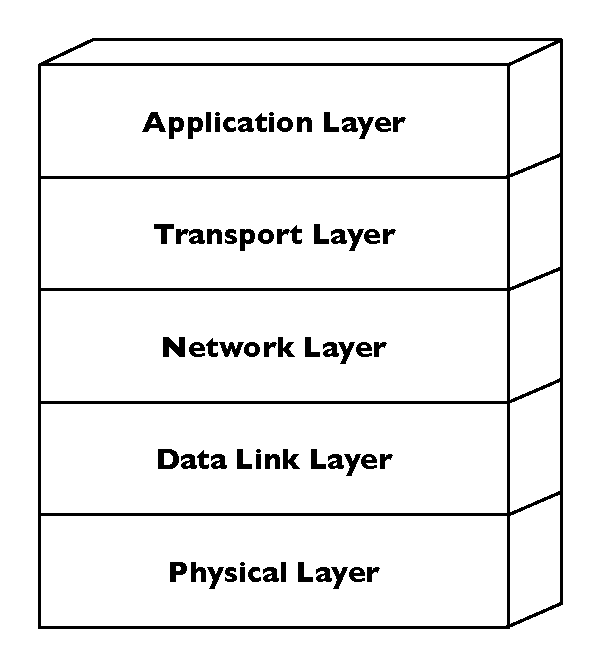
\includegraphics[scale=0.65]{img/ProtStack.eps}
\caption[WSN protocol stack]{WSN protocol stack (reproduced from \cite{SensorSurveyAkyildiz:2002})}
\label{Fig:ProtStack}
\end{figure}

\chapter{Background} \label{chap:background}

%% REWRITE!??

This chapter presents a brief discussion of the concepts and algorithms
that were used during the course of this work. 

This chapter begins with presentation of abstract data types and
discusses its applicability for WSNs. The chapter further presents distributed
abstract data types (DADTs) and concepts underlying them \cite{migliavacca_DADT:2006}.

This is followed by a brief presentation of the Logical Neighborhoods (LN) \cite{mottola_LNScoping:2006}, a mechanism that
enables routing and scoping in WSNs.  

%This
%chapter begins with an introduction to programming abstractions and continues
%with a discussion on their applications in WSN programming.

%This chapter further presents the concepts underlying Distributed Abstract Data
%Types (DADTs) \cite{migliavacca_DADT:2006}. This is followed by a presentation
%of the Logical Neighborhoods (LN) \cite{mottola_LNScoping:2006}, a mechanism
%that enables routing and scoping in WSNs. 

%The chapter then concludes with a
%description of the hardware platform - Sun Small Programable Object Technology
%(SPOT) \cite{simon_squawk:2006} - used to experimentally validate the
%implemented prototype in a real-world environment.

\section{Abstract Data Types}

An Abstract Data Type (ADT) is the depiction of a model that
presents an abstract view to the problem at hand. This model of a problem
typically defines the affected data and the identified operations associated with
those.

The set of the data values and associated operations, independent of any
specific implementation, is called an ADT \cite{NIST_website}. From the
application developer's point of view, the use of ADTs allows for the separation of
interfaces from specific implementations.

One may consider a \emph{stack} as a simple example of an ADT
\cite{guttag_ADTs:1977}. It can be represented through the stacked data, and a set of defined
operations that include \emph{push(data)}, \emph{pop()}, and \emph{top()}. It is intuitively clear that
several different implementations of an ADT may be defined using the proposed specification.


%\subsection{ADTs in WSNs} \label{subsubsec:ADTsinWSN}

The concept of ADTs has been successfully used in several different areas of
science. This idea clearly has found its applicability in WSNs, due to
possibility to separate interfaces provided by sensor nodes and their particular
implementations. 

%The rest of this section focuses on the application and extension of the concept of ADTs for use in WSNs.

A top-down aproach can be used to overview an abstraction of WSN and its parts.
Any WSN as described earlier, usually consists of a number of sensor nodes, where each
sensor node may include several sensors used to measure specific phenomenon.

\begin{figure}[h]
\centering
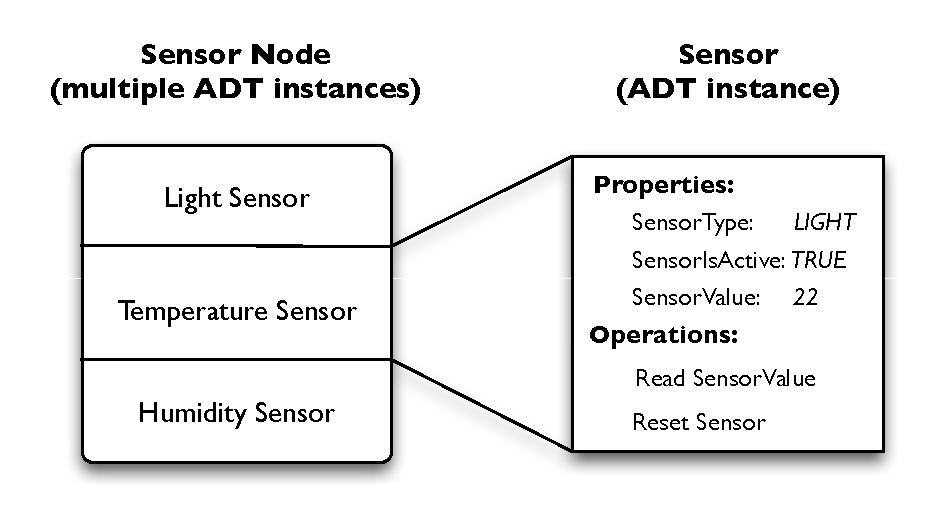
\includegraphics[scale=0.71]{img/ADTsMultipleInstances.eps}
\caption[Abstraction of sensor node through multiple ADTs]{Abstraction of sensor node through multiple ADTs}
\label{Fig:MultipleADTs}
\end{figure} 
  
Referring to the example in Figure \ref{Fig:MultipleADTs}, the ADT instance
\emph{Sensor} can be used to abstract different types of sensors that may be
present on a sensor node. It specifies that a \emph{Sensor} provides the list of
common properties and operations. By declaration of multiple such ADT instances,
the nature of the wireless sensor node can be abstracted, as can be seen in the
\emph{Sensor Node} entity shown in Figure \ref{Fig:MultipleADTs}. This then
allows the ADT instances to be used by the application developer at a later
point\footnote{Further details of ADT specification and instantiation are
provided in Section \ref{subsec:ADTSpecInst}}.

\section {Distributed Abstract Data Types} \label{sec:DADT}

Distributed Abstract Data Types present a new programming language construct
used to support distributed and context-aware applications. The concept of DADTs was
introduced in \cite{migliavacca_DADT:2006}, and based on the notion of ADTs,
which are divided into two classes - data and space ADTs. 
The rest of this section presents the concepts and provides the reader with the
relevant background and examples\footnote{The examples provided are adapted from \cite{migliavacca_DADT:2006}}.

\subsection{Data and Space ADTs} \label{subsubsec:DataAndSpaceADTs}

It is important to distinguish between data required by an application, and
the location, or space, where the providers of data reside. ADTs in WSNs can
provide not only the data from the sensor node, but also express a notion
of the ``computational environment'' hosting the data ADT.

Thus, ADTs be of two types:

\begin{itemize}
  \item \emph{Data ADTs}
  \item \emph{Space ADTs} 
\end{itemize}

\emph{Data ADTs} are ``conventional'' ADTs which encode application logic, such
as, for instance, allowing access to sensor data.

\emph{Space ADTs}, also known as \emph{sites}, are ADTs that provide an
abstraction of the computational environment (in the case of a WSN, a sensor
node) that ``hosts the data ADT'' \cite{migliavacca_DADT:2006}. The space ADT may
use different notions of space, such as physical location or network topology,
depending on application requirements as determined by the programmer.

\subsection{DADTs as an extension of ADTs} \label{subsec:DADTsConcepts}
Distributed ADTs (DADTs) are an extension of ADTs that make the state of multiple ADTs in a
distributed system collectively available.
\cite{migliavacca_DADT:2006}. 

\begin{figure}[h]
\centering
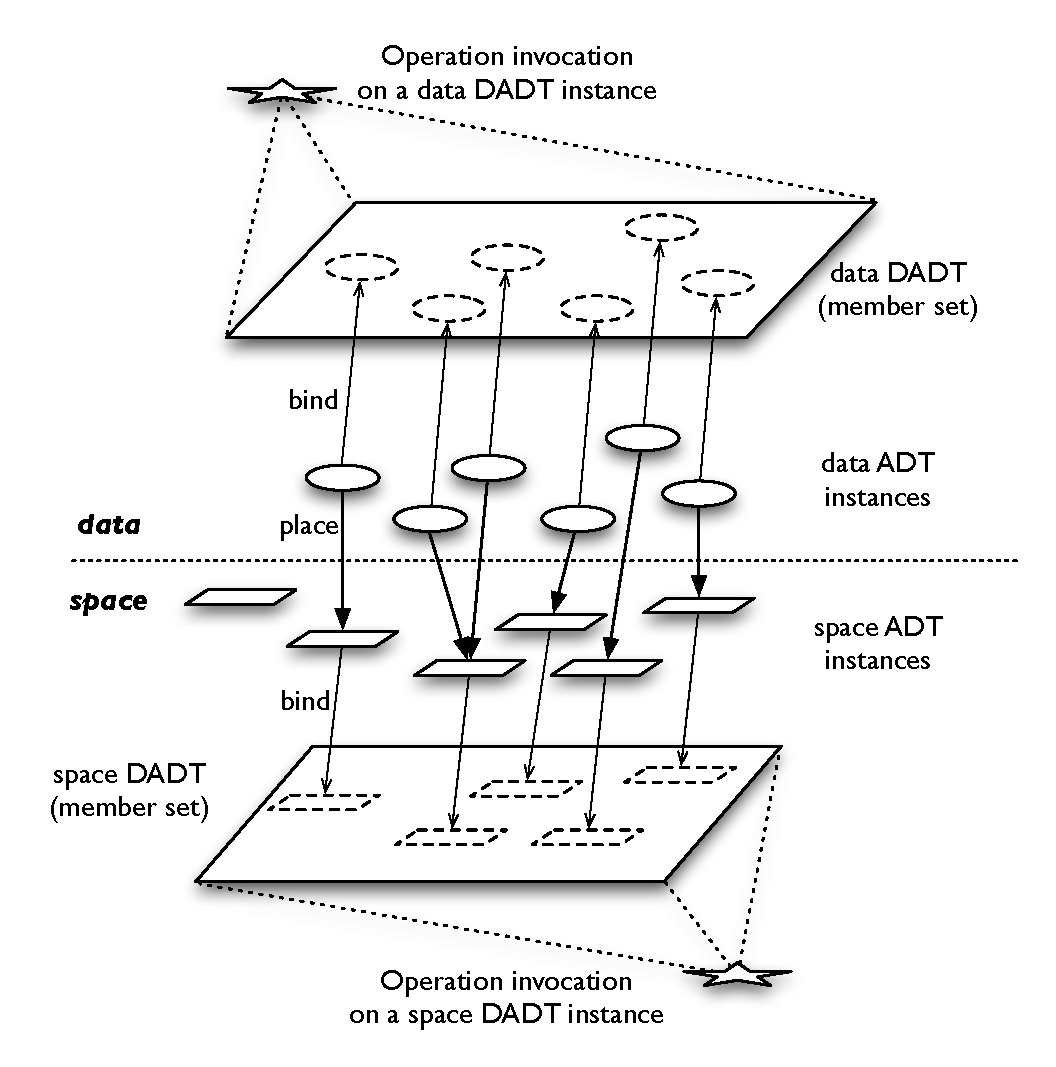
\includegraphics[scale=0.65]{img/DADTs.eps} 
\caption[Data and space in the DADT model]{Data and space in the DADT model (reproduced from 
\cite{migliavacca_DADT:2006})}
\label{Fig:DADTs}
\end{figure}

Similar to ADTs, DADTs 
provide specifications for distributed data, distributed operators, and 
constraints. The notion of space is extended to DADTs, and therefore DADTs can
either be (as it is shown in the Figure \ref{Fig:DADTs}):

\begin{itemize}
  \item \emph{Data DADT} that provide distributed access to a collection of data
  ADTs.
  \item \emph{Space DADT} that allows distributed access to a collection of
  space ADTs. 
\end{itemize}

The set of ADTs that are available for collective access using a DADT is called the \emph{member set} of
the DADT.

\subsubsection{DADT Operators and Actions} \label{subsubsec:OperatorsAndActions}

Operators are used in DADTs to declare distributed references to
the ADTs in the DADT member set. This reference conceals identities of individual ADT
instances from the application programmer. 

DADT operators may belong to one of the following types:

\begin{itemize}
  \item \emph{Selection Operators} that allow the performance of
  distributed operations on a subset of the instances in the member set.
  Examples of such operators could be \emph{all}, or \emph{any} selection
  operator, because they allow to declare a subset of the instances.

  \item \emph{Conditional Operators} that provide support for global
  conditions to be applied on the member set prior to the execution of the DADT
  operation. One of the examples of conditional operator is operator
  \emph{in}, that allows to check if one set of instances contains in another
  one.

  \item \emph{Iteration Operators} that allow iterating over the
  ADT instances in the set, and thus permit access to individual ADT instances.
  Examples of such operators are \emph{next}, \emph{previous}, \emph{last},
  \emph{first}, as they allow to address and iterate over the members of the
  set.
\end{itemize}

The DADT operators described above allow different way to access ADT
instance and execute one of the ADT operations defined in the
ADT specification.

Distributed appliation developer may require to implement more complicated
application logic, though it may happen that even available ADT operations
are not sufficient. In this case the special DADT construct, called DADT
action, can be used \cite{migliavacca_DADT:2006}. 

DADT actions are specified by the DADT type, but are executed similarly to ADT
 operation on remote ADT instances.

\subsubsection{Views} \label{subsubsec:views}

\emph{DADT Views} permit the definition of the scope of distributed operations
that the application requires to perform. This approach is particularly useful
when a distributed operation has to be executed only on a subset of the
member set of ADT instances. The concept of DADT Views is presented in Figure
\ref{Fig:DADT_Views}.

\begin{figure}[h]
\centering
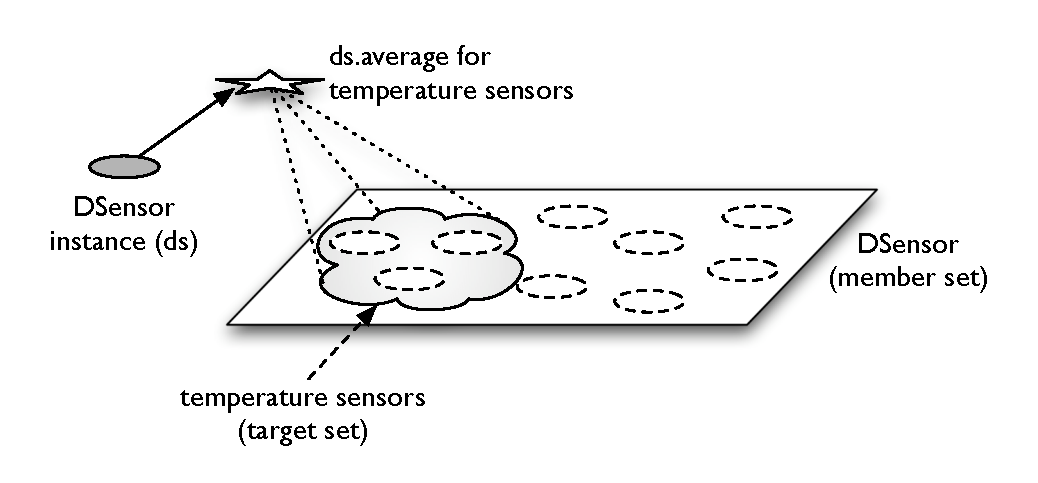
\includegraphics[scale=0.75]{img/DADT_Views.eps} 
\caption[DADT Views]{DADT views (reproduced from \cite{migliavacca_DADT:2006})}
\label{Fig:DADT_Views}
\end{figure}

The member set may be partitioned into DADT Views by using properties. A
\emph{Property} is a DADT characteristic that is defined in terms of an ADT's
data and operations, and is evaluated locally on the ADT instance
\cite{migliavacca_DADT:2006}. DADT View may either be:
\begin{itemize}
  \item \emph{Data View},
  \item \emph{Space View}.
\end{itemize}

Application developer should decide what could be the best
way to access the WSN. A Data DADT instance can be used to
operate on the distributed data and limit the scope using predicates over
DADT properties representing data, space, or both,
depending on the needs of the application. Similarly, any kind of view to
access the distributed representation of Space can be applied.

This section has presented concepts underlying the DADTs. A brief description
of the DADT prototype \cite{migliavacca_DADT:2006} will be presented further in
Section \ref{sec:DADTPrototype}.

\subsection {The DADT Prototype} \label{sec:DADTPrototype}

The DADT prototype implemented by Migliavacca et al \cite{migliavacca_DADT:2006}
was written in Java, and presents the design of a DADT specification language
that extends Java.

This section provides the reader with
further details on the concepts central to DADTs\footnote{All the DADT concepts presented below
are described using the DADT specification language.}, a description of the
existing DADT prototype \cite{migliavacca_DADT:2006}, and a discussion on its limitations.

\subsection{ADTs Specification and Instantiation} \label{subsec:ADTSpecInst}

As was mentioned in Section \ref{subsubsec:ADTsinWSN}, each sensor node
in a WSN can be abstracted using multiple ADT instances (see
Figure \ref{Fig:MultipleADTs}), and therefore conceal the details of sensor
node abstraction from the application developer. The code snippets below are
provided to illustrate these concepts.

The specification of a described ADT may be defined as a Java
class, as shown in Listing \ref{listing:ADTSpec}

\begin{lstlisting}[frame=trbl, basewidth={0.55em, 0.6em}, captionpos=b,
basicstyle=\ttfamily\footnotesize, breaklines, caption = Sensor ADT instances, label =
listing:ADTSpec]
class Sensor {
  //data properties of the sensor 
    int sensorType;
    double sensorReading;
    boolean active; 
  //operations that can be performed on the sensor  
    public double read(){ //read the sensor value.
    ...
    } 
    public void reset(){ //reset the sensor
    ...
    }    
\end{lstlisting}
 
This specification declares that a Sensor ADT instance should provide the following properties:
\begin{itemize}
\item an integer value to define the sensor type,
\item a double value that holds the sensor data, 
\item a boolean value that stores information about sensor's state of activity.
\end{itemize}
as well as operations that allow to \emph{Read} sensor data and \emph{Reset}
the sensor.

It is possible to define multiple such instances of this specification. For
example, the ADT instances for a given sensor node that has two kinds of sensors
- (a) a temperature sensor, and (b) a light sensor - may be defined using the ADT
specification described above, as shown in Listing \ref{listing:ADTInstances}. 
\begin{lstlisting}[frame=trbl, basewidth={0.55em, 0.6em}, captionpos=b,
basicstyle=\ttfamily\footnotesize, breaklines, caption = Sensor ADT instances, label =
listing:ADTInstances]
  // Temperature sensor ADT instance
    Sensor temperatureSensor = new Sensor(TEMPERATURE);
  // Light sensor ADT instance  
    Sensor lightSensor = new Sensor(LIGHT);
\end{lstlisting}

\subsection{DADT Specification and Instantiation} \label{subsubsec:dadtspecandinst}

The concept of DADTs was first introduced in Section \ref{sec:DADT}, and will
be extended in this chapter with examples of DADT specification and
instantiation.

DADT specifications can be best understood by carrying forward the example
described in Section \ref{subsec:ADTSpecInst}. To allow for collective access
to multiple ADT instances of the type specified in Listing
\ref{listing:ADTSpec}, a DADT \emph{DSensor} may be defined as shown in Listing
\ref{listing:DADTSpec}.   
 
\begin{lstlisting}[frame=trbl, basewidth={0.55em, 0.6em}, captionpos=b, 
basicstyle=\ttfamily\footnotesize, breaklines, caption = Data DADT 
specification (reproduced from \cite{migliavacca_DADT:2006}), label = listing:DADTSpec]
class DSensor distributes Sensor{	
  //properties:
    property isSensorType(int type);
    property isActive();

  // distributed operations:
    distributed double average()	
    distributed void resetAll();
}
\end{lstlisting} 
 
This DADT specification allows two simple distributed operations to be performed
on multiple data ADTs of type \emph{Sensor}:  
\begin{itemize}
\item \emph{resetAll()} 
\item \emph{average()} 
\end{itemize}

The \emph{resetAll()} operation is used to reset every sensor in the DADT member
set, or subset of ADT instances defined by a DADT View (see Section
\ref{subsubsec:views}).

The \emph{average()} operation allows for the calculation of the average of the readings of every
sensor in the member set, or the subset of it defined by the DADT view.

Additionally, the DADT specification  shown in Listing \ref{listing:DADTSpec}
declares two DADT Properties described later.

Listing \ref{listing:DADTInstance} shows how DADT specifications can be
instantiated as an object of a Java class, and be used to perform defined
distributed operations.

\begin{lstlisting}[frame=trbl, basewidth={0.55em, 0.6em}, captionpos=b, 
basicstyle=\ttfamily\footnotesize, breaklines, caption = DADT Instantiation 
(reproduced from \cite{migliavacca_DADT:2006}), label = listing:DADTInstance ]
  DSensor ds = new DSensor();
  ds.resetAll();
\end{lstlisting}

\subsection{Binding ADTs to DADTs}

As mentioned earlier in Section \ref{subsec:DADTsConcepts}, a DADT member set
consists of the set of ADTs that are available for collective
access, which, in the given example, is the collection of ADTs of type \emph{Sensor}.

An ADT instance is made part of the member set by binding it to the DADT type.
This can be done using a dedicated programming construct \emph{bind} as shown in
Listing \ref{listing:binding}, where the Sensor ADT defined in Listing
\ref{listing:ADTSpec} is bound to the DADT type \emph{DSensor} defined in Listing \ref{listing:DADTSpec}.
 
\begin{lstlisting}[frame=trbl, basewidth={0.55em, 0.6em}, captionpos=b, 
basicstyle=\ttfamily\footnotesize, breaklines, caption = Binding ADT instances to a DADT instance, label = listing:binding]
  bind(new Sensor(TEMPERATURE), "DSensor");
  bind(new Sensor(LIGHT), "DSensor");
  ...
\end{lstlisting} 

Binding of ADT instances takes place on the sensor device that holds sensors,
as those are abstracted into specific ADTs.

\subsection{Implementing DADT Operators and Actions}
\label{subsubsec:OperatorsAndActionsImpl}

The concepts of DADT Operators and Actions were already introduced in the
previous chapter (see Section \ref{subsubsec:OperatorsAndActions}). This
section describes the implementation of Operators and Actions in the DADT
prototype \cite{migliavacca_DADT:2006}.

\subsubsection{DADT Operators}
Listing \ref{listing:DADTOperator} extends the example first introduced in
Listing \ref{listing:DADTSpec}, and presents the use of the DADT selection
operator \emph{all}.

\begin{lstlisting}[frame=trbl, basewidth={0.55em, 0.6em}, captionpos=b, 
basicstyle=\ttfamily\footnotesize, breaklines, caption = Use of DADT Selection Operator, label = listing:DADTOperator]  
class DSensor distributes Sensor{
  ...
  distributed void resetAll(){
    (all in targetset).reset();
  }
}
\end{lstlisting}

The distributed operation \emph{resetAll} uses the selection operator 
\emph{all} in order to gain access to all ADT instances in the DADT
target set, and subsequently invokes the \emph{reset} operation on the ADT
instance. The \emph{reset} operation was declared in the ADT specification
shown in Listing \ref{listing:ADTSpec}.

\subsubsection{DADT Actions}
However, if the application developers finds the set of available ADT operations limited, he/she has the option of using DADT actions that are defined in the DADT type and executed locally on the ADT instance.

DADT actions do not necessarily consist only of single ADT operations, but can
also implement more complicated logic. For instance, a
\emph{reliableRead} action may be implemented that is capable of handling sensor read failures by means of performing multiple read attempts, failing which
a sensor node reset is performed (See Listing \ref{listing:DADTAction}).
 
\begin{lstlisting}[frame=trbl, basewidth={0.55em, 0.6em}, captionpos=b, 
basicstyle=\ttfamily\footnotesize, breaklines, caption = Use of DADT Action (reproduced from \cite{migliavacca_DADT:2006}), label = listing:DADTAction]  
class DSensor distributes Sensor {
  distributed double average(){
  ...  
  action double reliableRead(){
    double reading;
      int tries = 3;
      while (tries > 0){
        reading = local.read();  // use of ADT operation
        if (reading == ERROR) --tries;
        else break; 
      }
      if (reading == ERROR) {
        local.reset();
        reading = local.read();
      }
    }

    double[] sensorReadings = (all in targetset).reliableRead();
    ...
    // evaluation of the average value based on received readings	
    ...
    }
}
\end{lstlisting}

\subsection{DADT Views} \label{subsubsec:viewsImpl}

DADT Views are an effective tool for the application developer to
define the scope of a distributed operation. As was described in the Section
\ref{subsubsec:views}, DADT Views are created using DADT properties.

To continue to use the example running throughout this section, if the application programmer wishes to refer to a subset of temperature sensors from among the member set of ADT instances bound to the DADT type \emph{DSensor}, a data view \emph{TempSensors}, 
as shown in Listing \ref{listing:DADTview}, can be declared.
  
\begin{lstlisting}[frame=trbl, basewidth={0.55em, 0.6em}, captionpos=b, 
basicstyle=\ttfamily\footnotesize, breaklines, caption = Definition of DADT Data View, label = listing:DADTview ]  
dataview TempSensors on DSensor as isSensorType(TEMPERATURE) && isActive(); 
\end{lstlisting}

The DADT name \emph{DSensor} in this case refers to its member set, and 
the data view \emph{TempSensors} is defined as a subset of this member set and
consists only of sensor nodes with temperature sensors for which the evaluation of
both DADT properties (See Listing \ref{listing:DADTProperty}) \emph{isActive}
and \emph{isSensorType} return \emph{true}. 

\begin{lstlisting}[frame=trbl, basewidth={0.55em, 0.6em}, captionpos=b, 
basicstyle=\ttfamily\footnotesize, breaklines, caption = Definition of DADT Properties, label = listing:DADTProperty ]  
class DSensor distributes Sensor {
  property isSensorType(){
	 return (local.type == type);
  }
  property isActive() {
	return local.isActive();
  }
  ...
}

\end{lstlisting}

This section has described the DADT prototype presented in
\cite{migliavacca_DADT:2006}, which was modified and extended to use in WSNs. 
Chapter \ref{chap:design} provides further details about limitations of the
given prototype and presents the DADT/LN prototype. 

\section {Logical Neighborhoods} \label{LNDescription}

Typically, communication between WSN nodes is based on routing 
information between nodes by exploiting the communication radius of each node.
The notion of a node's physical neighbourhood - the set of nodes in the
network that fall within the communication range of a given node - is central to a mechanism of this nature.

However, in heterogenous WSN applications, the developer might require to
communicate with a specific subset of the network that is defined logically and
not physically. As an example of this, consider the following case. An
application that provides security in a high-risk environment by monitoring 
motion might require - in the event of a security alarm - all sensors at the
entrances to the guarded area to report about detected motion.
The sensors at the entrance form a logical neighbourhood in this case. However,
as the entrances may be widely separated, it is not for granted that these nodes
constitute part of a single physical neighbourhood.

The use of current WSN programming techniques to enable a mechanism of this
nature entails additional programming effort, because the developer has to deal
not only with the application logic, but also with the underlying problems of
transmitting messages to a specific logical neighbouhood while using lower layer
constructs that have no notion of this. This leads to increased code complexity
\cite{mottola_LN:2006}.

\begin{figure} 
\centering
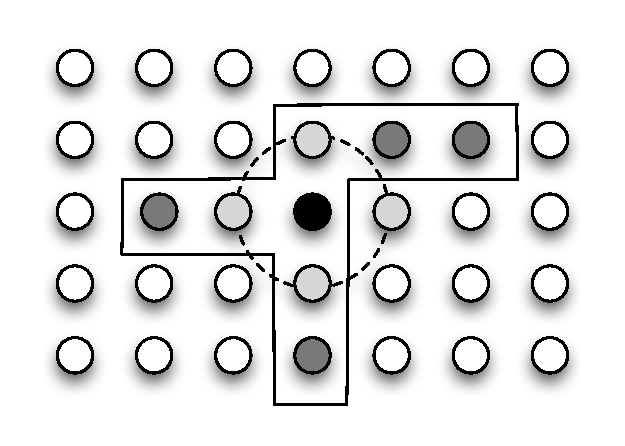
\includegraphics[scale=0.71]{img/LN_physical_vs_logical.eps} 
\caption[Difference between physical and logical neighborhoods]{Representation 
of logical and physical neighborhood of a given node. (reproduced from
\cite{mottola_LN:2006})}
\label{Fig:LN_physical_vs_logical}
\end{figure} 

Mottola and Picco \cite{mottola_LN:2006} suggest the addressing of the
aforementioned issues using \emph{Logical Neighbourhoods (LNs)}, an
abstraction that replaces the node's physical neighbourhood with a logical notion of
proximity. 

Figure \ref{Fig:LN_physical_vs_logical} provides comparison between
physical and logical neighbourhoods. The black node represents the node
that defines the sensor node with its neighbourhoods. The light grey nodes
connected by the dashed circle represent the physical neighborhood, whereas the
dark grey ones with the solid polygon represent (one of the nodes in) the
node's logical neighborhood.


Using this
abstraction, programmers can communicate with members of a LN using a simple message passing API,
thereby allowing for logical broadcasts. The implementation of this API is
supported by means of a novel routing mechanism devised specifically to support
LN communication. 

\subsection{The LN Abstraction}

LNs can be specified using a declarative language such as SPIDEY
\cite{mottola_LN:2006, mottola_LNScoping:2006}, and
involves the definition and instantiation of the \emph{node} and the
\emph{neighbourhood}. 

Nodes are a logical representation of the subset of a sensor node's state and
characteristics, and are used for the specification of an LN. Nodes are defined
in a node template and are subsequently instantiated, as shown in Listing \ref{listing:LN1}
   
A neighbourhood can be defined by applying predicates on the attributes defined
in the node template. The neighbourhood is defined using a neighbourhood
template, and subsequently instantiated.
   
\begin{lstlisting}[frame=trbl, basewidth={0.55em, 0.6em}, captionpos=b, 
basicstyle=\ttfamily\footnotesize, breaklines, caption = Node Definition and Instantiation, label = listing:LN1]  
node template Sensor
  static Function
  static Type
  dynamic BatteryPower
  dynamic Reading

create node ts from Sensor
  Function as "Sensor"
  Type as "Temperature"
  Reading as getTempReading()
  BatteryPower as getBatteryPower()
\end{lstlisting}


Listing \ref{listing:LN2} shows the definition and
instantiation of a
neighbourhood - based on the node template defined in Listing \ref{listing:LN1}
- which selects all temperature sensors where the reading exceeds a threshold.
 
\begin{lstlisting}[frame=trbl, basewidth={0.55em, 0.6em}, captionpos=b, 
basicstyle=\ttfamily\footnotesize, breaklines, caption = Neighbourhood Definition and Instantiation, label = listing:LN2]  
neighbourhood template HighTempSensors(threshold)
  with Function = "Sensor" 
      and Type  = "Temperature" 
      and Reading > Threshold

create neighbourhood HigherTemperatureSensors
  from HighTempSensors(threshold:45)
\end{lstlisting}

LN communication is enabled using a simple API that overrides the
traditionally used broadcast facility and makes it dependent on the (logical)
neighbourhood the message is addressed to \cite{mottola_LN:2006}. The underlying routing mechanism is presented in further
details in \cite{mottola_LN:2006, mottola_LNScoping:2006}.

\section{Summary}

This chapter presented an overview of the concepts, technologies, and hardware
underlying the work presented in this thesis. After underlining the need for the
use of programming models to increase the ubiquity of WSN use, this chapter
introduced a taxonomy of programming abstractions and placed the Distributed
Abstract Data Types programming abstraction used in this work within the
framework of the taxonomy. This was followed by a detailed discussion on Abstract
and Distributed Abstract Data Types used in the application layer of the
prototype produced during the course of this work, and the Logical Neighbourhood
routing mechanism used in the network and data link layers of the prototype. 


  
\chapter{Implementation} \label{chap:Implementation}

\begin{figure}
\centering
\label{Fig:DADTLN_architecture}
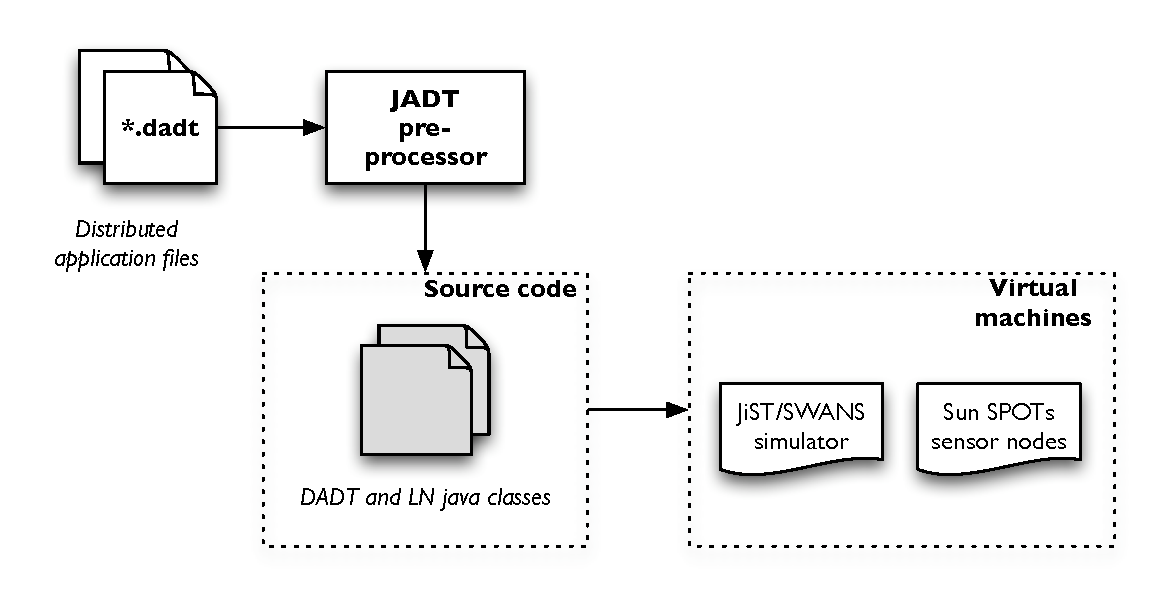
\includegraphics[scale=0.71]{img/DADTLN_architecture.eps} \caption[DADTLN
prototype architecture - to be renamed]{DADTLN prototype architecture - to
be moved to the other section}
\end{figure} 

\bibliography{references}
\bibliographystyle{acm}


\end{document}
